\documentclass[sigplan,9pt]{acmart}

\usepackage{booktabs} % For formal tables

\usepackage[utf8]{inputenc}
\usepackage{fullpage}

\usepackage{graphics}

\usepackage{graphicx}
\usepackage{subcaption}

\usepackage{multirow}

\usepackage{color}

\usepackage{soul}

%\usepackage{flushend}

%\usepackage{indentfirst}

\usepackage{amsthm}
\usepackage{amsmath,amssymb}
%\usepackage{mathrsfs}
\usepackage{mathtools}

\usepackage[noend]{algpseudocode}
\usepackage{algorithm}

\newcommand{\etal}{et~al.}
\algrenewcommand\algorithmicindent{3ex}%

% Copyright
\setcopyright{none}
%\setcopyright{acmcopyright}
%\setcopyright{acmlicensed}
%\setcopyright{rightsretained}
%\setcopyright{usgov}
%\setcopyright{usgovmixed}
%\setcopyright{cagov}
%\setcopyright{cagovmixed}


% DOI
%\acmDOI{10.475/123_4}

% ISBN
%\acmISBN{123-4567-24-567/08/06}

%Conference
\acmConference[CGO'18]{International Symposium on
Code Generation and Optimization}{2018}{} 
%\acmYear{1997}
%\copyrightyear{2016}
%
%\acmPrice{15.00}


\begin{document}
%\title{A work-based metric for efficiently applying online iterative optimisation}
\title{Online Iterative Optimisation\\Guided by Low Overhead Profiling}
%\titlenote{Produces the permission block, and
%  copyright information}
%\subtitle{Extended Abstract}
%\subtitlenote{The full version of the author's guide is available as
%  \texttt{acmart.pdf} document}


\author{Rodrigo C. O. Rocha}
%\authornote{Dr.~Trovato insisted his name be first.}
%\orcid{1234-5678-9012}
\affiliation{%
  \institution{University of Edinburgh, UK}
  %\streetaddress{P.O. Box 1212}
  %\city{Dublin} 
  %\state{Ohio} 
  %\postcode{43017-6221}
}
\email{r.rocha@ed.ac.uk}

\author{Pavlos Petoumenos}
%\authornote{The secretary disavows any knowledge of this author's actions.}
\affiliation{%
  \institution{University of Edinburgh, UK}
  %\streetaddress{P.O. Box 1212}
  %\city{Dublin} 
  %\state{Ohio} 
  %\postcode{43017-6221}
}
\email{ppetoume@inf.ed.ac.uk}

\author{Lu\'is F. W. G\'oes}
%\authornote{This author is the
%  one who did all the really hard work.}
\affiliation{%
  \institution{PUC Minas, Brazil}
  %\streetaddress{1 Th{\o}rv{\"a}ld Circle}
  %\city{Hekla} 
  %\country{Iceland}
}
\email{lfwgoes@pucminas.br}

\author{Murray Cole}
\affiliation{
  \institution{University of Edinburgh, UK}
  %\streetaddress{P.O. Box 5000}
}
\email{mic@inf.ed.ac.uk}

\author{Zheng Wang}
\affiliation{%
  \institution{Lancaster University, UK}
  %\city{Moffett Field}
  %\state{California} 
  %\postcode{94035}
}
\email{z.wang@lancaster.ac.uk}

\author{Hugh Leather}
\affiliation{%
  \institution{University of Edinburgh, UK}
  %\streetaddress{8600 Datapoint Drive}
  %\city{San Antonio}
  %\state{Texas} 
  %\postcode{78229}
}
\email{hleather@inf.ed.ac.uk}

%\author{John Smith}
%\affiliation{\institution{The Th{\o}rv{\"a}ld Group}}
%\email{jsmith@affiliation.org}

%\author{Julius P.~Kumquat}
%\affiliation{\institution{The Kumquat Consortium}}
%\email{jpkumquat@consortium.net}

% The default list of authors is too long for headers}
\renewcommand{\shortauthors}{R. Rocha et al.}


\begin{abstract}
Efficiently selecting the best combination of compiler optimisations for a program
remains an open problem due to their complex interaction and the large optimisation search space.
Iterative optimisation techniques, which consist of iterating
over this large space searching for the best optimisation,
has the ability to adapt to new platforms, programs and workload while still
having a systematic and simple optimisation process.
Although some recent work have studied the impact of using multiple
input datasets for performing iterative optimisation, applying this
technique in an online scenario still poses some challenges.

In this paper, our main goal is to enable iterative optimisation in
online scenarios with the restriction of executing distinct inputs
only once.
In order to address this challenge,
we propose a the use of a work-based metric that allows for comparing different
combination of compiler optimisations even when executed with distinct inputs.
Because of its online nature, we also propose a relaxed instrumentation
that performs low overhead profiling of the amount of work executed, while
being able to trade-off between accuracy and overhead in a controlled manner.
\end{abstract}

%
% The code below should be generated by the tool at
% http://dl.acm.org/ccs.cfm
% Please copy and paste the code instead of the example below. 
%
\begin{CCSXML}
<ccs2012>
<concept>
<concept_id>10011007.10011006.10011041</concept_id>
<concept_desc>Software and its engineering~Compilers</concept_desc>
<concept_significance>500</concept_significance>
</concept>
<concept>
<concept_id>10011007.10011006.10011041.10011043</concept_id>
<concept_desc>Software and its engineering~Retargetable compilers</concept_desc>
<concept_significance>500</concept_significance>
</concept>
</ccs2012>
\end{CCSXML}

%\ccsdesc[500]{Software and its engineering~Compilers}
%\ccsdesc[500]{Software and its engineering~Retargetable compilers}


\keywords{Iterative Optimisation, Profiling, Relaxed Instrumentation}

\maketitle

\section{Introduction}

Modern optimising compilers
have reached a high level of sophistication,
providing a large number of optimisations.
Because of the unpredictability of optimisation
interactions, in addition to the growing complexity
of processor architectures and applications,
the correct choice of optimisations and their ordering
can have a significant impact on the performance of the
code being optimised~\cite{pan06,fursin07,kulkarni12}.

Each of these optimisations interacts with the code in complicated ways,
depending on all other optimisations and the order they were applied to
the code being optimised.
Understanding the interactions of optimisations is very important
in determining a good solution to the phase-ordering problem~\cite{touati06,kulkarni12}.
Because of all those dependences and interactions, although
most compiler optimisations yield significant improvements
in many programs, the potential for performance degradation in
certain program patterns is known to compiler writers and many users~\cite{pan06,zhou12,kulkarni12}.
%Traditional compilers typically apply the same set of optimisation in a fixed order to all functions in a program, without regard the code being optimised.

Efficiently selecting the best combination of compiler optimisations
for a given program or program section remains an open problem.
Compiler writers typically use a combination of experience and insight to construct
the default sequences of prearranged optimisations found in compilers.
However, these default pre-arranged set of optimisations do not include all possible optimisations
and they are always applied in the same pre-defined fixed order, without regard the code being optimised~\cite{pan06,cavazos07,zhou12,kulkarni12}.
%in hopes that a programmer will know which combination of optimisations will benefit their code~\cite{pan06,cavazos07,zhou12,kulkarni12}.

A well known compilation technique that addresses this challenge is iterative
optimisation.
Iterative optimisation has the ability to adapt to new
platforms, program and workload while still
having a systematic and simple optimisation process.
Iterative optimisations repeatedly evaluate a large number
of compiler optimisations until the best combination is
found for a particular program~\cite{fursin07,chen10}.
The main challange concerning iterative optimisation is the need for quickly
exploring such a large optimisation space~\cite{fursin07,cavazos07,zhou12}.

Until recently, most of existing work  had been focusing
on finding the best optimisation through repeated runs using a single input.
Although they demonstrate the potential of iterative optimisation,
in real scenarios the user rarely executes the same input dataset multiple times~\cite{bodin98,kisuki99,stephenson03,kulkarni04,agakov06}.
Applying iterative optimisation in light of a single input may not result in good performance when executing the optimised code with different inputs.

Most of real world applications are complex enough 
so that a single input case does not capture the whole
range of possible scenarios and program behaviour~\cite{haneda06,fursin07,chen10,chen12a}.
Because programs can exhibit behaviours that differ greatly depending on the input,
%This is something that is well known when writing test
%cases for correctness.
%We can extend the same argument when optimising the code for performance.
using a single input for iterative optimisation can produce poor performance when executed with different inputs.

Recent work have been studying
the impact of using multiple input datasets
for performing iterative optimisation.
This previous work suggests that optimising based on a representative range of input datasets
allows for selecting a robust compiler optimisation 
that produces good performance in real scenarios where
the input is expected to change constantly~\cite{haneda06,fursin07,chen10,chen12a,chen12b,fang15,mpeis16}.
Their results show that a limited number of input datasets may be sufficient to
obtain a well optimised program for a wider range of different inputs~\cite{haneda06,fursin07,chen10,chen12a}.

Finding such a robust combination of compiler optimisations by means of iterative optimisation across a large range of inputs
may be very time consuming.
In order to speed up this process we intend to reduce the number of actual executions during the exploration
of the optimisation space without much degradation of the final selected optimisation.

\begin{figure}[htb]
    \centering
    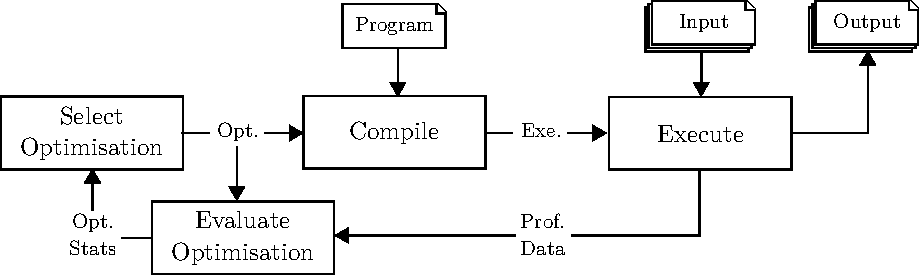
\includegraphics[width=\linewidth]{figs/diagram}
    \caption{Overview of the execution engine for applying iterative optimisation.}
    \label{fig:diagram}
\end{figure}

In this paper, our main goal is to enable iterative optimisation in
\textit{online} scenarios with the restriction of executing distinct inputs
only once, while targeting optimal performance across different inputs.
This online aspect is usually found in mobile and data centre
platforms~\cite{chen12b,fang15,mpeis16}, where the goal is to optimise
programs based on the workload of a particular user (or group of users)
between executions.

Measuring just execution time, for example, is useful only if the
amount of work is constant between executions with different inputs.
For this reason, we propose the use of a work-based metric in order
to compare the performance of different optimisations across 
multiple executions of the program with distinct inputs.

Because of the restriction of not repeating inputs, we instrument the program
for measuring the amount of work it performed during its execution.
Having a low overhead instrumentation is essential in this online scenario for
two main reasons:
$(i)$ the user is directly affected by large overheads;
$(ii)$ a highly intrusive instrumentation can havea significant impact on the
effect of the optimisations.

Our main contributions are the following:
\begin{itemize}
\item The use of a work-based metric in order to enable online iterative
optimisation by comparing different combination of compiler optimisations even
when executed with distinct inputs.
\item We propose a relaxed instrumentation for low overhead profiling, with a controlled
trade-off between accuracy and overhead.
\end{itemize}

\section{Related Work}

Chen~\etal~\cite{chen10,chen12a} evaluate the effectiveness of iterative
compilations across a large number of input test cases.
Their main motivation is to answer the question:
\textit{How data input dependent is iterative optimisation?}
Their results show that it is possible to find a combination of compiler optimisations
that achieves at least 86\% of the maximum speedup across all input test cases.
These optimal combinations are program-specific and yield average
speedups up to 3.75$\times$ over the highest optimisation level of compilers.

When optimising a program, the main method for iterative optimisation used by Chen~\etal~\cite{chen10,chen12a}
evaluates each combination of compiler optimisations across all the available inputs, i.e.,
if $N$ is the number of input test cases and $M$ is the total number of combinations of compiler optimisations,
they perform a total of $O(NM)$ runs of the program being optimised.
Furthermore, they use a pre-defined set of only 300 different combinations of compiler optimisations,
which represents a very small sample of the optimisation search space for most modern compilers, e.g.
LLVM has 56 distinct optimisation passes and GCC has about 47 high-level (SSA form) optimisation passes and
about 25 low-level (RTL) optimisation passes, which in both cases result in much more than $2^{50}$ distinct
combinations of compiler optimisations, without considering repetition.

Recent work~\cite{chen12b,fang15} have applied the same idea of performing
input-dependent iterative optimisation to distributed applications on data centres.
In summary, each worker receives a subset of the input dataset, called the evaluation dataset,
to perform an \textit{online} iterative optimisation of the code being executed.
Each worker performs the same the method for iterative optimisation used by Chen~\etal~\cite{chen10,chen12a},
i.e., they evaluate each combination of compiler optimisations across all the evaluation dataset.
However, because the optimisation is performed online, they usually consider a small evaluation dataset
and a small number of compiler optimisations.

Fursin~\etal~\cite{fursin07} addressed the problem of comparing the effect of two optimisations
on two distinct inputs. For that purpose, they proposed to use instruction per cycle (IPC) as the metric for performing such comparison.
Their result show that using IPC seems promising as a robust metric for iterative optimisation
across large input datasets.
However, 
some specific optimisation techniques may affect the use of IPC as a robust metric, and specially
IPC has been shown to provide poor performance estimation for multi-threaded programs~\cite{alameldeen06,eyerman08}.
In particular, IPC can give a skewed performance measure if threads spend time in \textit{spin-lock loops}
or other synchronisation mechanisms. 
Some existing work on performance assessment suggest that
total execution time should be used for measuring performance of multi-threaded programs~\cite{alameldeen06,eyerman08}.
Aalameldeen and Wood~\cite{alameldeen06} in particular suggest that a simple work-related metric should be used
if the unit of work is representative enough.
Work-related metrics have already been largely used for measuring performance of throughput-oriented applications,
for other applications, however, choosing an appropriate unit of work can be more challanging~\cite{alameldeen06}.

\section{Work-based Metric} \label{sec:metric}

A possible candidate for a work-based metric, borrowing from Physics,
is using the concept of \textit{average power}, i.e. the amount of
\textit{work}, $\Delta W$, performed during a period of time, $\Delta t$.
\[
   P_{avg} = \frac{\Delta W}{\Delta t}
\]

%The hypothesis is that, given two optimisations $o_1$ and $o_2$,
%a program compiled with optimisation $o_2$ would \textit{consistently} perform better
%than when it is compiled with $o_1$, i.e., $o_1 \tilde{<}_p \, o_2$,
%if it performs more \textit{work} per unit of time when compiled with $o_2$
%instead of $o_1$. 
By measuring the amount of \textit{work} done per unit of time we reduce
the impact of input-dependent aspects and focus instead on the efficiency
of the optimised program.
For this metric, the main challange is to precisely define what
represents \textit{work}.

%For that purpose, we intend to use profiling
%techniques to measure the input size and amount of computation
%performed on the execution path triggered by the input~\cite{ball94,ball96,zaparanuks12,coppa14}.

%In addition to being useful for speeding up iterative optimisation across a large
%number of different inputs, this metric based on comparing work-based efficiencies could
%potentially be used for applying iterative optimisation \textit{online}. 
%However, the overhead for estimating the amount of \textit{work} must be low
%enough for the performance gains to be beneficial.

Previous work have proposed profiling-based mechanism to estimate
input sizes~\cite{zaparanuks12,coppa14}.
Coppa~\etal~\cite{coppa14} in particular propose the concept of
\textit{read memory size} for automatically estimating the size of the input
passed to a routine, where \textit{read memory size} represents the number of
distinct memory cells first accessed by a read operation.
In other words, the \textit{read memory size} metric measures the size of the 
useful portion of the input's memory footprint.
However, because we are interested in the amount of computational work performed
in respect of a given input, the memory footprint of the input may not always
have a direct correspondence to  the amount of computational work.

Goldsmith~\etal~\cite{goldsmith07} use \textit{block frequency} as the
measure for performance for empirically describing the asymptotic behaviour
of programs, which is known as empirical computational complexity.
Block frequency is a relative metric that represents the number of times a
basic block executes~\cite{ball94,ball96}. 
They argue in favour of block frequency due to its portability, repeatability
and exactness, since it does not suffer from timer resolution problems or
non-deterministic noises.
Block frequency also has the advantage of being efficiently profiled by means
of automatic code instrumentation~\cite{knuth73,ball94}.

However, in the context of comparing different optimisations,
although block frequency would be able to capture aspects of optimisations
that simplify the control-flow graph (CFG), measuring work at the basic block
resolution would not capture effects of optimisations at the instruction level.
Because of that, we extend the idea of using basic block frequency to measure
computational work by also considering the computational cost of each
basic block. The computational cost of a basic block is given by weighing
the instructions that it contains.

We model the computational work $\Delta W$ as a linear equation based on
block frequency information and a cost-model of the instruction set.
\[
\Delta W = \varepsilon + \sum_{B} w(B)f(B)
\]
where $f(B)$ represents the frequency of basic block $B$
and $w(B)$ represents the computational work of executing $B$.
We define the work of a basic block $B$ as the sum of the cost
of its instructions, i.e.,
\[
w(B) = \sum_{i} w_i N_B(i)
\]
where $w_i$ is the cost of instruction $i$ and $N_B(i)$ is the number of
occurrences of instruction $i$ in basic block $B$.

In this simplified model, we consider that $w_i$ is constant across all
programs and executions in the given target platform.
However, $N_B(i)$ is program dependent but constant across executions,
while $f(B)$ is both program and execution dependent, since $f(B)$ can
change when executing with different inputs.
In other words, $N_B(i)$ is a static value known at compile-time and 
$f(B)$ is a dynamic value known only at run-time.
%If we define $x_i$ as
%\[
%x_i = \sum_{B\in P} N_B(i)f(B)
%\]
%we can write our definition of work $\Delta W$ as the following linear equation
%\[
%\Delta W = \varepsilon + \sum_{i\in I} w_i x_i
%\]

%\subsection{Linear regression}
%
%\begin{figure}[htb]
%    \centering
%    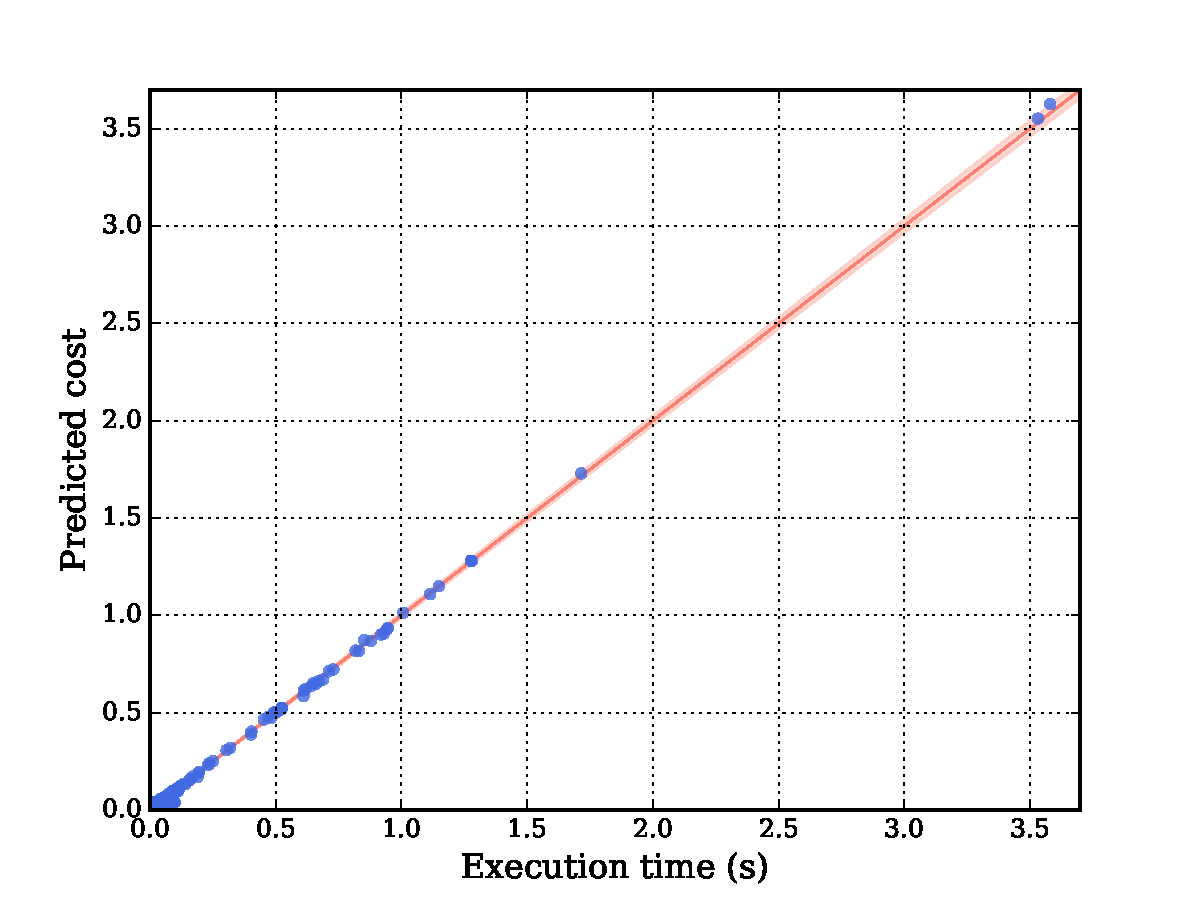
\includegraphics[width=\linewidth]{figs/cost-model.pdf}
%    \caption{Comparison between the naive and optimal instrumentation with no compiler optimisation.} %, i.e., compiled with \textbf{\texttt{-O0}}.}
%    \label{fig:cost-model}
%\end{figure}
%mse 0.000145373168444
%mae 0.00737261168981
%mae* 0.0033892281406
%mape 75.2924320971
%corr (0.99946441743545622, 0.0)

\section{Instrumentation}

In this section we describe how the computation of the work-metric can be
performed during runtime by means of instrumenting the code.
%with the necessary computation for the work metric, $\Delta W$, as described in Section~\ref{sec:metric}.
Because we define work as a linear equation on the block frequency counters,
it is possible to embed its computation into the execution of the program.
A naive instrumentation would consists basically of having a global counter
that starts with the interception value, $\varepsilon$, and each basic block
increments its own cost into the global counter. Although this instrumentation
is easily implemented, it inserts a large amount of overhead into the program.

In 1973, Donald Knuth~\cite{knuth73} provided an optimal algorithm for
profiling block frequency, inserting fewer probes than the previously described
naive instrumentation that was commonly used in practice~\cite{knuth71}.
Forman~\cite{forman81} proposed further overhead reductions by placing the
probes in basic blocks that are less likely to be executed based on static
heuristics.
Ball and Larus~\cite{ball94} offered a detailed discussion comparing
two approaches for optimally profiling block frequency, namely,
placing probes on the vertices or the edges of the control-flow graph (CFG).
They show that the edge-based approach produces optimal placement of probes.

Ball and Larus~\cite{ball94} show that a set of edges represents the minimum
number of probes for profiling block frequency if and only if the complementary
set of edges forms a spanning tree.
The instrumentation optimises the placement of the probes with respect to a
weighing that assigns a non-negative value to each edge in the CFG.
The cost of profiling a set of edges is proportional to the sum of the weights
of the edges.
These weights can be obtained either by empirical measurements or heuristic
estimations.
In order to minimise the profiling cost, the instrumentation computes the
maximum spanning tree for avoiding probing in frequently executed edges.
Although this instrumentation algorithm is proved to produce the optimal
placement of probes for well-structured CFGs, it may produce sub-optimal
placement for some unstructured CFGs.

Once we have the maximum spanning tree, probes are placed on any edge not in 
the spanning tree. Figure~\ref{fig:cfg-example} shows an example of a CFG
with a maximum spanning tree represented by the black edges, while the edges 
highlighted in red represent the placement of the probes.

\begin{figure}[htb]
\centering {
  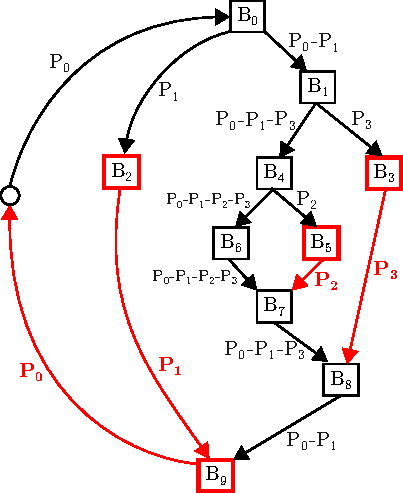
\includegraphics[scale=0.9]{figs/cfg-example.pdf}\\\vspace{1ex}
  \resizebox{0.45\textwidth}{!}{
  %\scalebox{0.8}{
     \begin{minipage}{0.5\textwidth}
     Instrumented value for each probe $P_i$:
     \begin{align*}
     w(P_0) &= w(B_0) + w(B_1) + w(B_4) + w(B_6) + w(B_7) + w(B_8) + w(B_9)\\
     w(P_1) &= w(B_2) - w(B_1) - w(B_4) - w(B_6) - w(B_7) - w(B_8)\\
     w(P_2) &= w(B_5) - w(B_6)\\
     w(P_3) &= w(B_3) - w(B_4) - w(B_6) - w(B_7)
     \end{align*}
     \end{minipage}
  }
}
  \caption{Example of a CFG with its minimum spanning tree in black and the
   basic blocks highlighted in red represent the instrumented basic blocks with
   the placement of the probes.}
  \label{fig:cfg-example}
\end{figure}

In contrast to the naive instrumentation where each basic block records only
its own amount of work, with the optimal profiling, the instrumented basic blocks
need record an aggregated value of work that represents a path in the CFG.
These values are constructed with some instrumented basic blocks speculatively
assuming some paths while other probes correct when these assumptions are wrong
(see for example $w(P_0)$ and $w(P_1)$ in Figure~\ref{fig:cfg-example}).

\begin{algorithm}[h]
  \caption{Pseudocode of the data-flow analysis for assigning the values computed
  in each probe of the instrumentation for the profiling of the work metric.}
  \label{alg:populateEdgeInfo}
  \begin{algorithmic}
    \Function{\textrm{populateEdgeInfo}}{$G$}
    
    \For{\textbf{each} $e \in $ \textrm{instrumentedEdges}($G$) }
       \State $B_I \gets $ \textrm{instrumentedBlock}($e$)
       \State $inc[e] \gets \{ B_I \}$
       \State $dec[e] \gets \{ \}$
       \State $known[e] \gets $ \textbf{true}
    \EndFor

    \State $changed \gets $ \textbf{true}
    \While{$changed$}
       \State $changed \gets $ \textbf{false}
	   \For{\textbf{each} $B \in V(G)$}
          \State $uIn \gets $ \textrm{unknownIn}($known, G, B$)
          \State $uOut \gets $ \textrm{unknownOut}($known, G, B$)
		  \If{$uIn=0$ \textbf{and} $uOut=1$}
             \State $changed \gets $ \textbf{true}
		     \State $incOut \gets \{\}$
			 \State $decOut \gets \{\}$
		     \For{$B_p\in$ \textrm{predecessors}($G, B$)}
			    \State $incOut \gets incOut \bigcup inc[(B_p,B)]$
			    \State $decOut \gets decOut \bigcup dec[(B_p,B)]$
			 \EndFor
		     \For{$B_s\in$ \textrm{successors}($G, B$)}
			    \State $incOut \gets incOut \cup dec[(B,B_s)]$
			    \State $decOut \gets decOut \cup inc[(B,B_s)]$
			 \EndFor
		     \For{$B_s\in$ \textrm{successors}($G, B$)}
			    \If{\textbf{not} $known[(B,B_s)]$}
			       \State $inc[(B,B_s)] \gets incOut\setminus{decOut}$
			       \State $dec[(B,B_s)] \gets decOut\setminus{incOut}$
			       \State $known[(B,B_s)] \gets$ \textbf{true}
				\EndIf
			 \EndFor
		  \EndIf
		  \If{$uIn=1$ \textbf{and} $uOut=0$}
             \State $changed \gets $ \textbf{true}
		     \State $incIn \gets \{\}$
			 \State $decIn \gets \{\}$
		     \For{$B_s\in$ \textrm{successors}($G, B$)}
			    \State $incIn \gets incIn \cup inc[(B,B_s)]$
			    \State $decIn \gets decIn \cup dec[(B,B_s)]$
			 \EndFor
		     \For{$B_p\in$ \textrm{predecessors}($G, B$)}
			    \State $incIn \gets incIn \bigcup dec[(B_p,B)]$
			    \State $decIn \gets decIn \bigcup inc[(B_p,B)]$
			 \EndFor
		     \For{$B_p\in$ \textrm{predecessors}($G, B$)}
			    \If{\textbf{not} $known[(B_p,B)]$}
			       \State $inc[(B_p,B)] \gets incIn\setminus{decIn}$
			       \State $dec[(B_p,B)] \gets decIn\setminus{incIn}$
			       \State $known[(B_p,B)] \gets$ \textbf{true}
				\EndIf
			 \EndFor
		  \EndIf
	   \EndFor
    \EndWhile
    \EndFunction
  \end{algorithmic}
\end{algorithm}

Because the algorithm for the optimal placement of the probes is proved to
uniquely compute the block frequencies by propagating the probe counts,
we adapt this algorithm in order to compose the aggregated values that will
be instrumented in each probe, based on our model of computational work,
$\Delta W$, derived from the basic block frequencies (see Section~\ref{sec:metric}).
We perform a similar propagation of the probes in a symbolic fashion,
as illustrated in Figure~\ref{fig:cfg-example}.
This symbolic propagation of the probes is implemented by the data-flow analysis
described in Algorithm~\ref{alg:populateEdgeInfo}, and the final aggregated values
are extracted from the edge information as described by Algorithm~\ref{alg:instrValue}.

The data-flow analysis in Algorithm~\ref{alg:populateEdgeInfo} keeps two sets
for each edge, namely, the increment and the decrement sets.
We consider that both sets represent the \textit{edge expressions} shown in Figure~\ref{fig:cfg-example},
for which we define a \textit{symbolic sum} by computing the union of the increment
and decrement sets, respectively, with the appropriate cancellation of common elements.
This data-flow analysis is based on the invariant that the symbolic sum
of all the incoming edges must equals the symbolic sum of the outgoing
edges. For example, the symbolic sum of the incoming edges of the basic
block $B_8$ is $P_0 - P_1$, where $P_3$ is cancelled out.

%By construction, 
%the \textit{symbolic experssions} of a basic block, i.e., 
%the \textit{symbolic sum} of the incoming edges (or outgoing edges) of a basic block,
%has the following properties:
%\begin{enumerate}
%\item Probes in the increment set either (post-)dominates or is (post-)dominated by the given basic block;
%\item Probes in the decrement set are (post-)dominated by the probes in the increment set;
%\item Probes in the decrement set and the given basic block are in exclusive paths
%      from the virtual node of the CFG to the (post-)dominators in the increment set;
%\end{enumerate}
%From property (1) it follows that whenever the given basic block is executed,
%exactly one of the probes in the increment set is executed.
%From properties (2) and (3), it follows that whenever a probe in the decrement set
%is executed, although the given basic block is not executed, one of the probes
%in the decrement set is executed.

Algorithm~\ref{alg:instrValue} reads the edge information for each
basic block by computing the symbolic sum of their respective incoming
edges (or outgoing edges).
From these \textit{edge expressions}, we are able to compose the aggregated
value of the probes.
The positive terms in the edge expression of a basic block indicate that the
amount of work of this basic block will be incremented in the probes represented
by these positive terms, similarly, the negative terms indicate that the amount
of work of this basic block will be decremented in the probes represented by
these negative terms.
For example, because the edge experssion for the basic block $B_8$ is
$P_0 - P_1$, the amount of work of $B_8$, denoted by $w(B_8)$,
is incremented in probe $P_0$ and decremented in $P_1$.

\begin{algorithm}[h]
  \caption{Pseudocode that describes how the edge information is used in order to extract
           the value that will be computed in a given instrumented basic block $B_I$.
           This algorithm could equally be implemented based on the predecessors.}
  \label{alg:instrValue}
  \begin{algorithmic}
    \Function{\textrm{instrValue}}{$G, B_I, inc, dec$}
	\State $v \gets 0$
    \For{\textbf{each} $B \in V(G)$}
	   \State $inc_B \gets \{\}$
	   \State $dec_B \gets \{\}$
%	   \For{$B_p\in$ \textrm{predecessors}($G, B$)}
%	      \State $inc_B \gets inc_B \bigcup inc[(B_p,B)]$
%	      \State $dec_B \gets dec_B \bigcup dec[(B_p,B)]$
%	   \EndFor
	   \For{$B_s\in$ \textrm{successors}($G, B$)}
	      \State $inc_B \gets inc_B \bigcup inc[(B,B_s)]$
	      \State $dec_B \gets dec_B \bigcup dec[(B,B_s)]$
	   \EndFor
	   \If{ $B_I \in inc_B\setminus{dec_B}$}
	      \State $v \gets v + w(B)$
	   \EndIf
	   \If{ $B_I \in dec_B\setminus{inc_B}$}
	      \State $v \gets v - w(B)$
	   \EndIf
	\EndFor
    \Return $v$
    \EndFunction
  \end{algorithmic}
\end{algorithm}

\subsection{Relaxed Instrumentation}

Although the optimal instrumentation significantly reduces the profiling overhead
when compared to the naive instrumentaion, from an average overhead of 79\% to 13\%,
in some critical cases, even the optimal instrumentation can have an overhead
of about 70\% (see benchmark \texttt{adpcm\_d} in Figure~\ref{fig:overhead-O3}).
In order to further reduce the overhead in these critical cases, we propose a relaxed instrumentation by trading off accuracy and overhead.

%\begin{figure*}[htb]
%    \centering
%    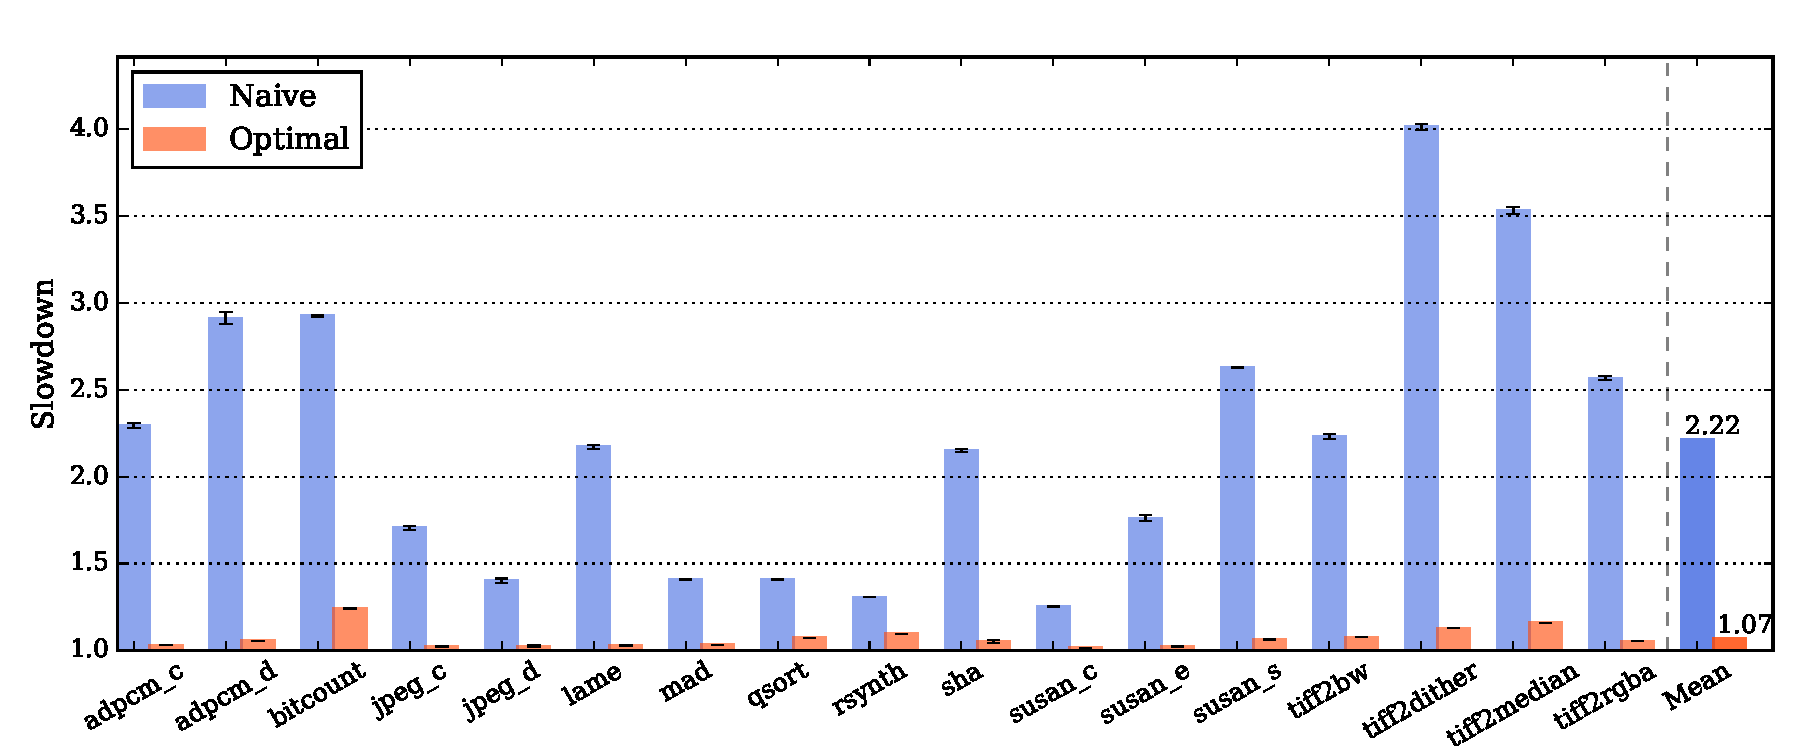
\includegraphics[width=\textwidth]{figs/overhead-O0.pdf}
%    \caption{Comparison between the naive and optimal instrumentation
%              with no compiler optimisation.}
%    \label{fig:overhead-O0}
%\end{figure*}

%Define an extended DAG of a CFG as a directed graph which may contain cycles
%if they have known constant trip counts.

The relaxed instrumentation performs a post-processing on the resulting instrumentation
of the optimal algorithm. 
The relaxation starts by extracting \textit{extended} DAGs (directed acyclic graphs)
from the CFG, as illustrated in Figure~\ref{fig:cfg-relax-example}.
Each loop (and the outer most region of the function) represents an extended DAG
where any inner loop is considered to never execute, i.e. only the headers of the
inner loops are included into the extended DAG.

%
%LLVM has a Scalar Evolution Analysis which is used primarily to analyse expressions
%involving induction variables in loops~\cite{pop05}.
%An induction variable is a variable that is increased or decreased by a fixed amount
%on every iteration of a loop or is a linear function of another induction variable.
%
%This Scalar Evolution Analysis provides a way to compute \textit{small} constant
%trip counts (where \textit{small} is defined by a threshold).

\begin{figure}[h]
  \centering
  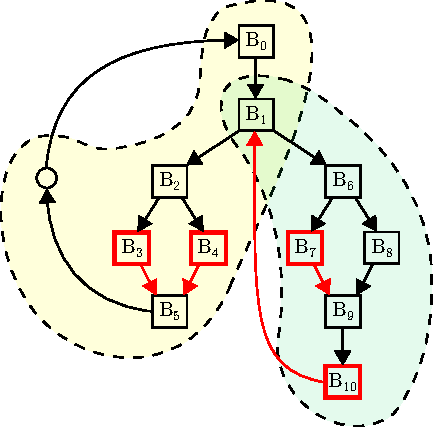
\includegraphics[scale=0.9]{figs/cfg-relax-example.pdf}
  \caption{Example of a CFG containing a loop and its decomposition into extended DAGs
           when applying the relaxation.}
  \label{fig:cfg-relax-example}
\end{figure}

For every extended DAG with a set of probes $\{P_0, P_1, \ldots, P_k\}$,
we relax the instrumentation accuracy by selecting a subset of the probes to be removed,
subject to the maximum allowed percentage error, $M$.

We model the relaxation as a 0-1 Knapsack problem:
\[
%\textrm{maximise } \sum_{i=0}^{k} f(I_i)c(I_i)x_i
\textrm{maximise } \sum_{i=0}^{k} f(P_i)x_i
\]
\[
\textrm{subject to } \sum_{i=0}^{k} \varepsilon(P_i)x_i \leq M \textrm{ and } x_i\in\{0,1\}
\]
%$c(I_i)$ is the relative overhead of the instrumentation on the instrumented basic block,
where $f(P_i)$ is the execution frequency of the instrumented basic block $P_i$
,$\varepsilon(P_i)$ is the percentage error of removing probe $P_i$ relative
to the minimum work value possible to compute in the extended DAG,
and $x_i$ denotes the probes selected for removal.
Because the percentage error is computed based on the path with the minimum
amount of work, $\varepsilon(P_i)$ represents the maximum error possible
that would be incurred when removing probe $P_i$.
Furthermore, by constraining the percentage error of every extended DAG below a
given threshold we guarantee that the final error of the relaxation will always
be bounded by the threshold.

While the optimal placement of probes tries to place probes in edges that are
less likely to be executed, the relaxation focus on removing probes that are
more likely to be executed.
The necessary block frequency information for optimising both the placement of
probes can be acquired from profiles of previous executions of the program or
by a static heuristic of the CFG during compilation.

For our experiments, we implemented two solvers for the 0-1 Knapsack problem:
the optimal brute-force solver;
the greedy heuristic based on sorting the items ~\cite{dantzig57}.
We use the brute-force solver for DAGs with a small number of probes and
the greedy heuristic when the number of probes is greater than a threshold.
Some of the benchmarks have DAGs with several hundreds of probes, which could
result in a long compilation time.

\section{Experimental Evaluation}

In this section we discuss our experimental evaluation.
First we describe the benchmarks with datasets used in the experiments.
Afterwards, we discuss our results concerning the instrumentations for profiling
our work metric.
Finally we present the results of the online iterative optimisation.

We implemented the instrumentations in LLVM 4.0.
The target platform is a Linux-4.4.27 system with an Intel Core i7-4770 3.40GHz
Skylake~CPU with 16~GiB RAM.

\subsection{Benchmarks}

%Iterative optimisations is essentially based on repeatedly trying
%out a large number of compiler optimisations until the best
%combination of compiler optimisations is found for a particular program.
%Our main goal is to speed up iterative optimisation while targeting
%optimal performance across large input datasets.

For the experimental evaluation we have used a subset of the \textit{KDataSets} benchmark suit,
which is the same benchmark and dataset suit used by Chen~\etal~\cite{chen10,chen12a}.
The KDataSets contains 1000 different inputs for each one of its benchmark programs.
These benchmarks cover a broad spectrum of application scenarios, ranging from simple
embedded signal-processing tasks to common mobile-phone and desktop tasks.
The different inputs try to capture distinct characteristics in terms of workload sizes
and how these workloads exercise different control flow paths.
A summary of the benchmark and dataset suit is shown in Table~\ref{tab:kdatasets}.

\begin{table}[h]
\centering
\scalebox{.8}{
\begin{tabular}{|c|c|c|c|}
\hline
\textbf{Program} & \textbf{LOC}    & \textbf{Input file size}            & \textbf{Input description}              \\ \hline % Domain
bitcount      & 460    &  -                         & Numbers: random                \\ \hline
qsort         & 154    & 32K-1.8M                   & 3D coordinates                 \\ \hline
%dijkstra      & 163    & 0.06K-4.3M                 & Adjacency matrices             \\ \hline
%patricia      & 290    & 0.6K-1.9M                  & IP and mask pairs              \\ \hline
jpeg\_d       & 13501  & 3.6K-1.5M                  & JPEG images                    \\ \hline
jpeg\_c       & 14014  & 16K-137M                   & PPM images                     \\ \hline
tiff2bw       & 15477  & \multirow{4}{*}{9K-137M}   & \multirow{4}{*}{TIFF images}   \\ \cline{1-2}
tiff2rgba     & 15424  &                            &                                \\ \cline{1-2}
tiffdither    & 15399  &                            &                                \\ \cline{1-2}
tiffmedian    & 15870  &                            &                                \\ \hline
susan\_c      & 1376   & \multirow{3}{*}{12K-46M}   & \multirow{3}{*}{PGM images}    \\ \cline{1-2}
susan\_e      & 1376   &                            &                                \\ \cline{1-2}
susan\_s      & 1376   &                            &                                \\ \hline
%mad           & 2358   & 28K-27M                    & MP3 audios                     \\ \hline
lame          & 14491  & 167K-36M                   & WAVE audios                    \\ \hline
adpcm\_c      & 210    & 167K-36M                   & WAVE audios                    \\ \hline
adpcm\_d      & 211    & 21K-8.8M                   & ADPCM audios                   \\ \hline
%gsm           & 3806   & 83K-18M                    & Sun/NeXT audios                \\ \hline
%ghostscript   & 99869  & 11K-43M                    & Postscript files               \\ \hline
%ispell        & 6522   & \multirow{3}{*}{0.1K-42M}  & \multirow{3}{*}{Text files}    \\ \cline{1-2}
%rsynth        & 4111   &                            &                                \\ \cline{1-2}
rsynth        & 4111   &                            &  Text files                    \\ \hline %%%%%% copied line
%stringsearch  & 338    &                            &                                \\ \hline
%blowfish\_e   & 863    & 0.6K-35M                   & Files of any format            \\ \hline
%blowfish\_d   & 863    & 0.6K-35M                   & Encrypted files                \\ \hline
%pgp\_e        & 19575  & 0.6K-35M                   & Files of any format            \\ \hline
%pgp\_d        & 19575  & 0.4K-18M                   & Encrypted files                \\ \hline
%rijndael\_e   & 952    & 0.6K-35M                   & Files of any format            \\ \hline
%rijndael\_d   & 952    & 0.7K-35M                   & Encrypted files                \\ \hline
sha           & 197    & 0.6K-35M                   & Files of any format            \\ \hline
%CRC32         & 130    & 0.6K-35M                   & Files of any format            \\ \hline
%bzip2e        & 5125   & 0.7K-57M                   & Files of any format            \\ \hline
%bzip2d        & 5125   & 0.2K-25M                   & Compressed files               \\ \hline
\end{tabular}
}
\caption{Description of the KDataSets with 1000 inputs for each benchmark (Chen~\etal~\cite{chen10,chen12a}).}
\label{tab:kdatasets}
\end{table}

\subsection{Evaluation of the Instrumentation}

\begin{figure*}[htp]
    \centering
    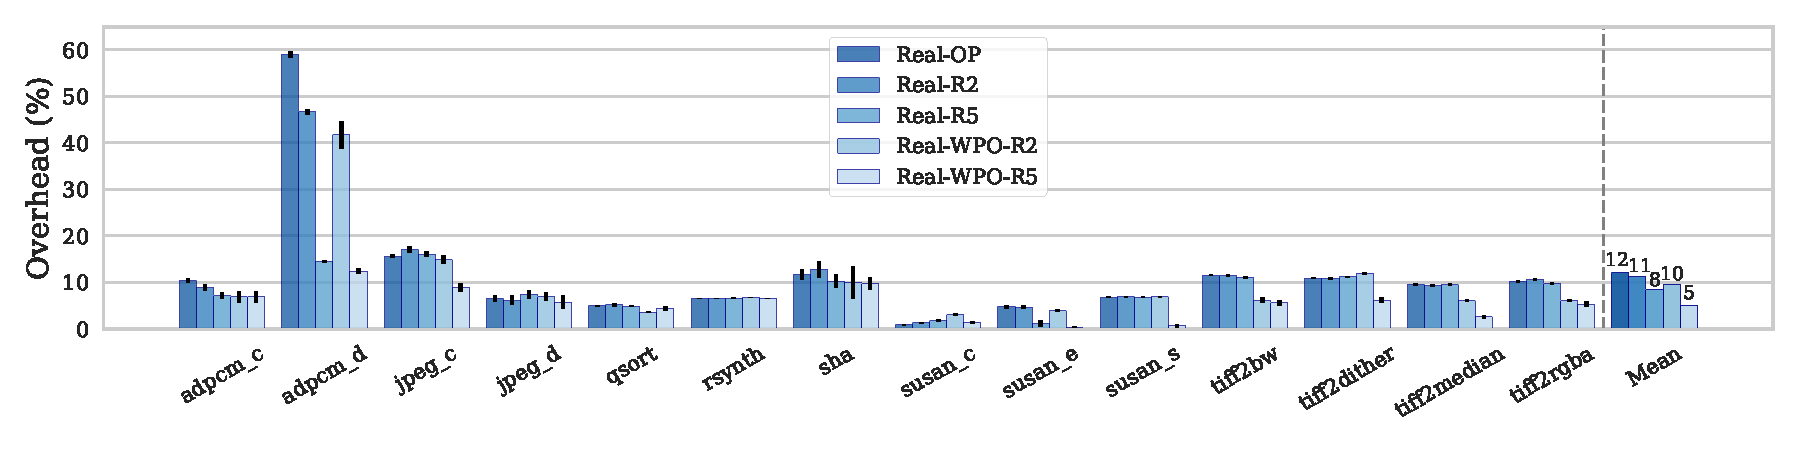
\includegraphics[width=\textwidth]{figs/overhead-O3.pdf}
    \caption{Overhead of the instrumentations compiled with {\texttt{-O3}}.}
    \label{fig:overhead-O3}
\end{figure*}

Figure~\ref{fig:instr} shows percentage of instrumented basic blocks
for the optimal and the relaxed instrumentation with different relaxation
thresholds. The naive instrumentation always has 100\% of the basic blocks
instrumented, by definition.

\begin{figure*}[htp]
    \centering
    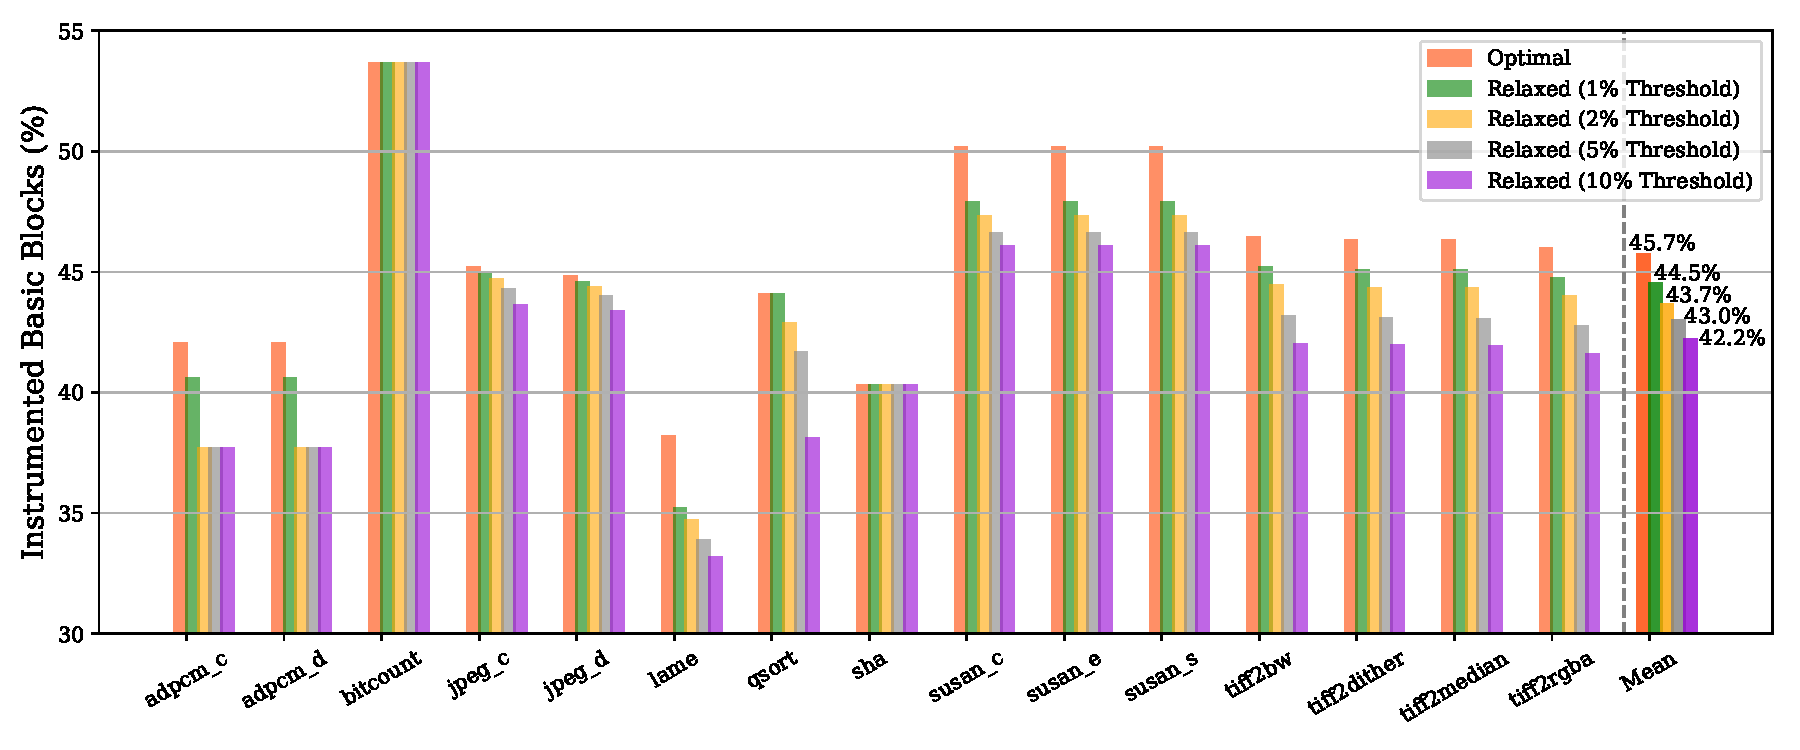
\includegraphics[width=\textwidth]{figs/instr.pdf}
    \caption{Percentage of instrumented basic blocks
for the optimal and the relaxed instrumentation with different relaxation
thresholds.}
    \label{fig:instr}
\end{figure*}

The \texttt{adpcm\_d} benchmark is the most critical case amongst the
used benchmarks, with a overhead of about 66\% with the optimal instrumentation.
This benchmark consists mainly of a single hot loop with several branches
inside it.
The relaxation algorithm is able to reduce this overhead down to about 52\%
(with an error threshold of 1\%) and 19\% (with an error threshold of 2\%)
by removing only one and two probes from the hot loop, respectively.
These two removed probes were placed in branches, inside the hot loop, with
a high probability of being taken, but with a small contribution to the work
measured in the loop.

%In this section we discuss the three baseline implementations that will
%be used for assessing the quality of the proposed metric.

%\vspace{1ex}
%\noindent \textbf{Iterative optimisation over a single input}

%Most of the existing iterative optimisation studies find the
%best optimisation though repeated runs on the same input.
%Although this approach will usually lead to sub-optimal performance
%across large input datasets, it provides a good baseline when considering
%the complexity and resonably low compile-time regarding
%iterative optimising compilers.
%If $M$ is the total number of combinations of compiler optimisations,
%this approach requires $O(M)$ runs of the program being optimised.
%We can consider two main scenarios:
%\textit{($i$ - best case scenario)}
%after selecting the optimisation over each individual input,
%consider the one with best performance across the whole input dataset;
%\textit{($ii$ - expected scenario)}
%after selecting the optimisation over each individual input,
%consider the average case of their performance across the whole input dataset.

%\vspace{1ex}
%\noindent \textbf{Iterative optimisation across large input datasets}

%Recent work on iterative optimisation have been targeting optimisation
%across multiple inputs~\cite{fursin07,chen10,chen12a}.
%If $N$ is the number of input test cases and $M$ is the total number of combinations of compiler optimisations,
%they perform a total of $O(NM)$ runs of the program being optimised.
%Similarly to what have been discussed previously,
%there are different ways for how to determine the optimal
%combination of compiler optimisations across multiple inputs.
%It is possible to tune the selection of the program-optimal combination
%to minimise risk or to maximise average performance.
%A compromise-based selection criterion could be to maximise average speedup
%with minimised variance.

%\vspace{1ex}
%\noindent \textbf{Iterative optimisation based on the IPC metric}

%While the previous two baselines addresses two opposite aspects of iterative optimisation,
%namely, compile-time efficiency and performance of the generated code,
%we also intend to compare against IPC as the competing baseline.
%The main reason for comparing against IPC is because it has been proposed as a metric
%for comparing the performance of two optimisations running on two distinct inputs.
%If $M$ is the total number of combinations of compiler optimisations,
%this approach requires $O(M)$ runs of the program being optimised.

\subsection{Evaluation of the Online Iterative Optimisation}

\begin{itemize}
\item Oracle-RM executes the program twice, for each input, and then measuring
the real speedup for each compiler optimisation and uses the real speedup for
selecting the best optimisation.
\item Oracle-PP represents the \textit{perfect} non-intrusive profiling by also
executing the program twice, once for estimating the amount of work and the
second for measuring its execution time.
This version uses the work-based metric, $\frac{\Delta W}{\Delta t}$, during
the iterative optimisation search.
\end{itemize}



\begin{figure*}[htb]
    \centering
    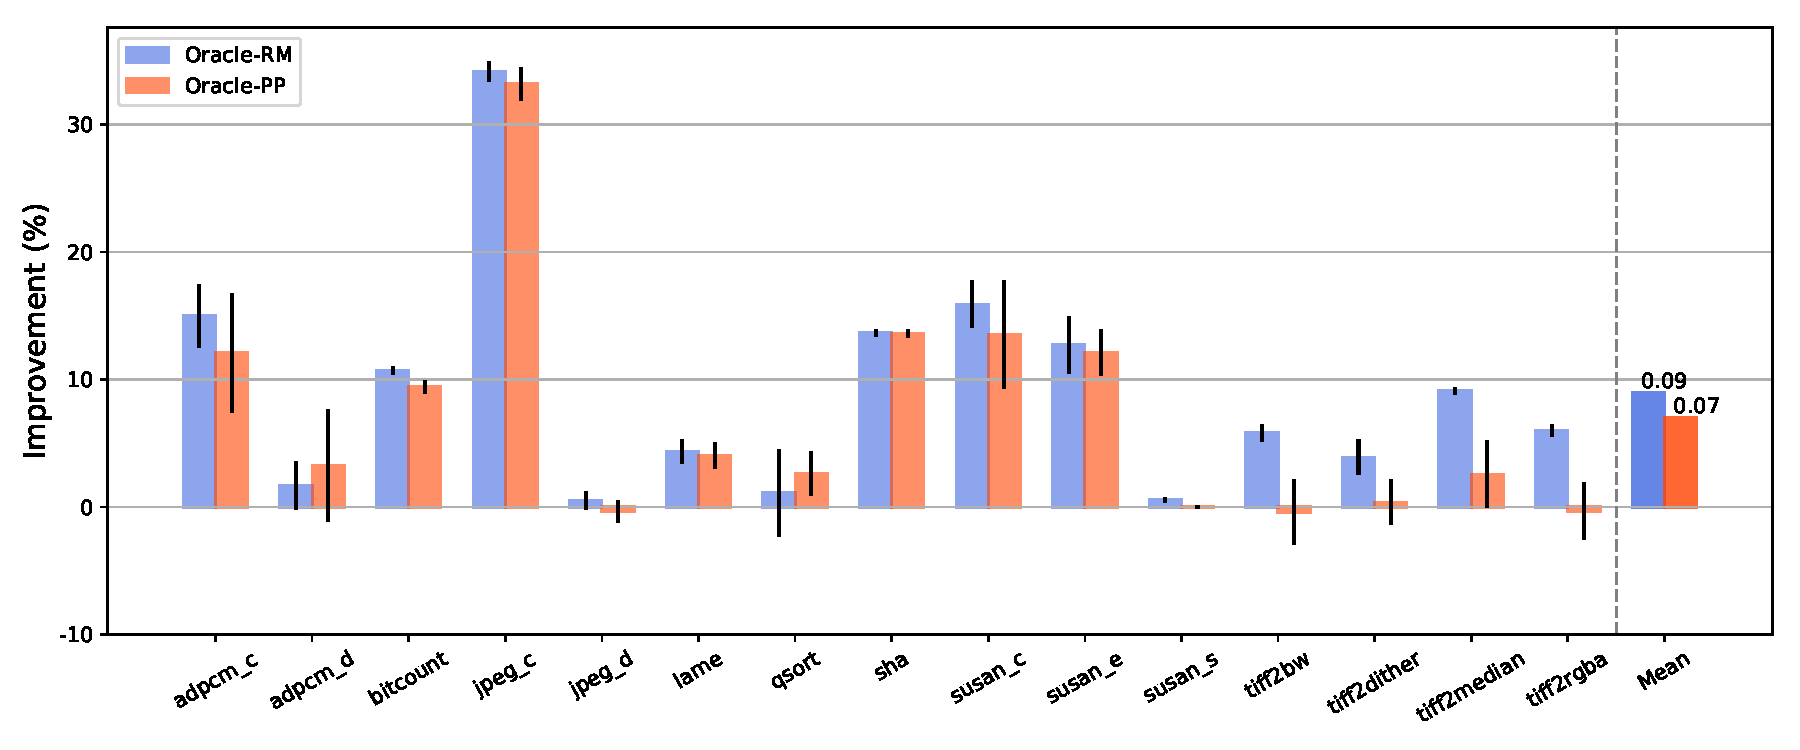
\includegraphics[width=\textwidth]{figs/speedups.pdf}
    \caption{Speedups observed with the online iterative optimisation.}
    \label{fig:speedups}
\end{figure*}

%\begin{figure*}[htb]
%    \centering
%    \includegraphics[width=\textwidth]{figs/profiled-speedups.pdf}
%    \caption{Speedups observed with the online iterative optimisation if we
%             consider the instrumentation overhead.}
%    \label{fig:profiled-speedups}
%\end{figure*}

%\subsubsection{Contribution of individual optimisation passes}
%
%Figure~\ref{fig:flagsfreq} shows an aggregated view of the final combination
%of compiler optimisations that were selected by iterative optimisation search.
%The figure presents the individual optimisation passes with at least 1\% of
%frequency in the selected combination of compiler optimisations that improved
%the performance over {\texttt{-O3}}.
%
%\begin{figure*}[htb]
%    \centering
%    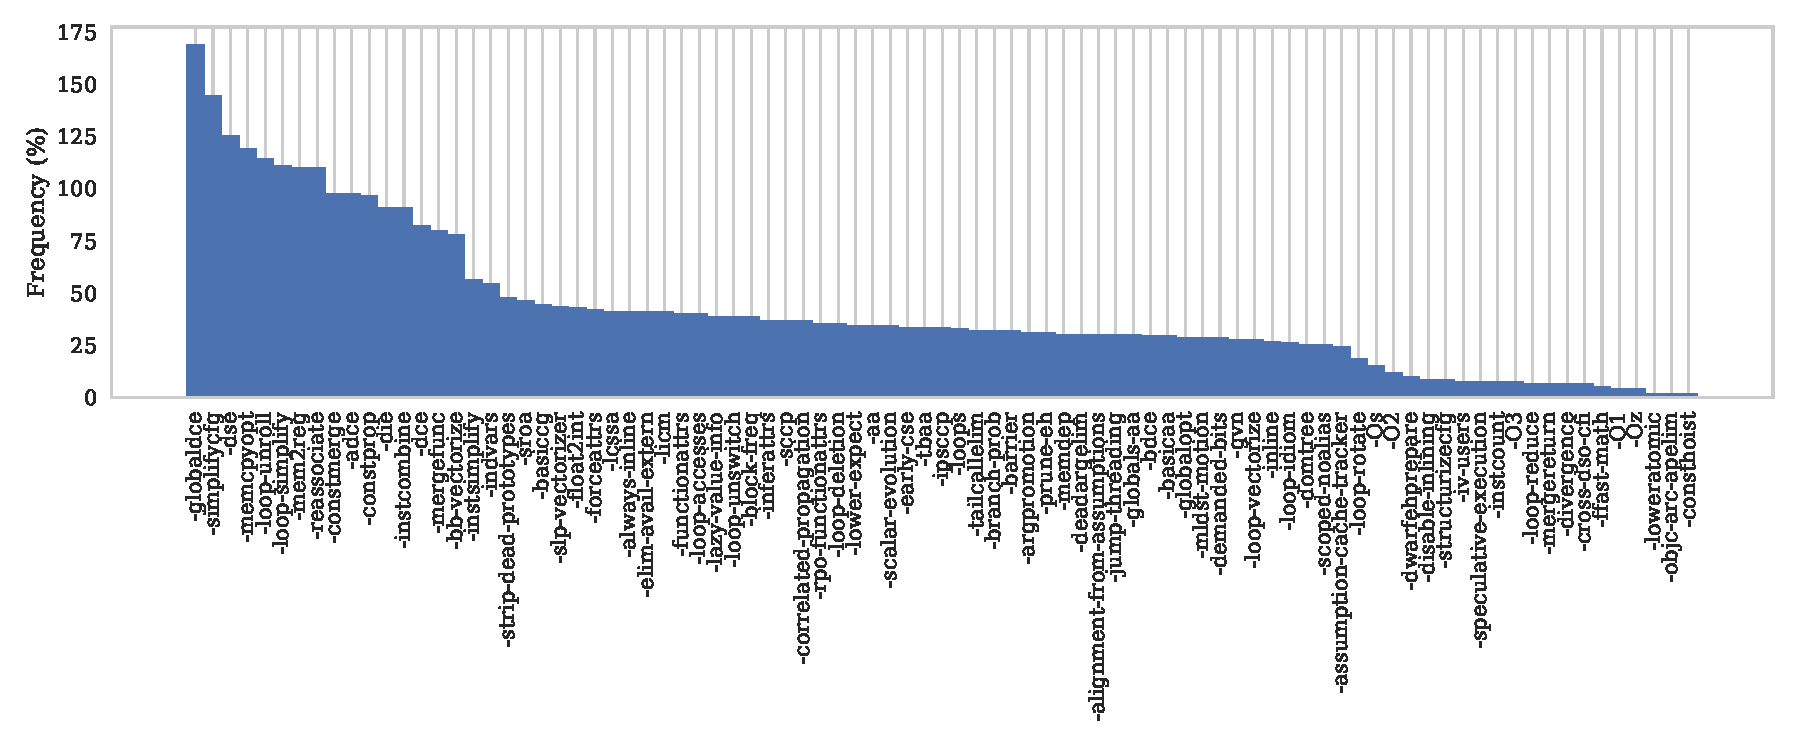
\includegraphics[width=\textwidth]{figs/flagsfreq.pdf}
%    \caption{Frequency of individual optimisation passes on the final selected 
%             compiler optimisations of the iterative optimisation search over
%             all benchmarks.}
%    \label{fig:flagsfreq}
%\end{figure*}

\section{Conclusion and Future Work}

Our proposed technique for relaxed instrumentation can also be applied for similar
profiling scenarios, such as profiling empirical computational complexity~\cite{goldsmith07,zaparanuks12,coppa14}.

\section*{Acknowledgments}

%\textbf{Acknowledge the partial support by EPSRC}.

This work was supported by the UK Engineering
and Physical Sciences Research Council (EPSRC) under grants
EP/L01503X/1 for the University of Edinburgh, School
of Informatics, Centre for Doctoral Training in Pervasive
Parallelism, % (\url{http://pervasiveparallelism.inf.ed.ac.uk/}),
and also by the Institute for Computing Systems Architecture (ICSA)
in the School of Informatics at the University of Edinburgh.

\bibliographystyle{ACM-Reference-Format}
\bibliography{ref} 

\end{document}
